\section{Navigation Methodology}
This section elaborates on how to equip the visuomotor control policy with the capacity to perform mobile manipulation tasks.

\subsection{ViNT Navigation Foundation Model}
To endow the trained visuomotor policy with navigation capabilities, \ourshort integrates an image-goal navigation foundation model~\cite{shah2023gnm,shah2023vint,sridhar2024nomad} that operates solely on RGB inputs and supports long-horizon, in-the-wild navigation. This framework allows for a seamless and low-cost fusion of manipulation and navigation modules, without necessitating additional fine-tuning of either component. We choose ViNT~\cite{shah2023vint} for achieving image-goal robotic navigation.  ViNT searches for the goal observations in the constructed topological map and computes a sequence of relative waypoints based on the current and goal observations, which are then translated into actions to control the low-level mobile controller. We deploy ViNT on our customized robotic system, operating at a frequency of 7.6 Hz. ViNT not only enables long-range, in-the-wild navigation but also demonstrates effective zero-shot generalization capability without necessitating model fine-tuning. 
\begin{figure*}[t]
  \centering
  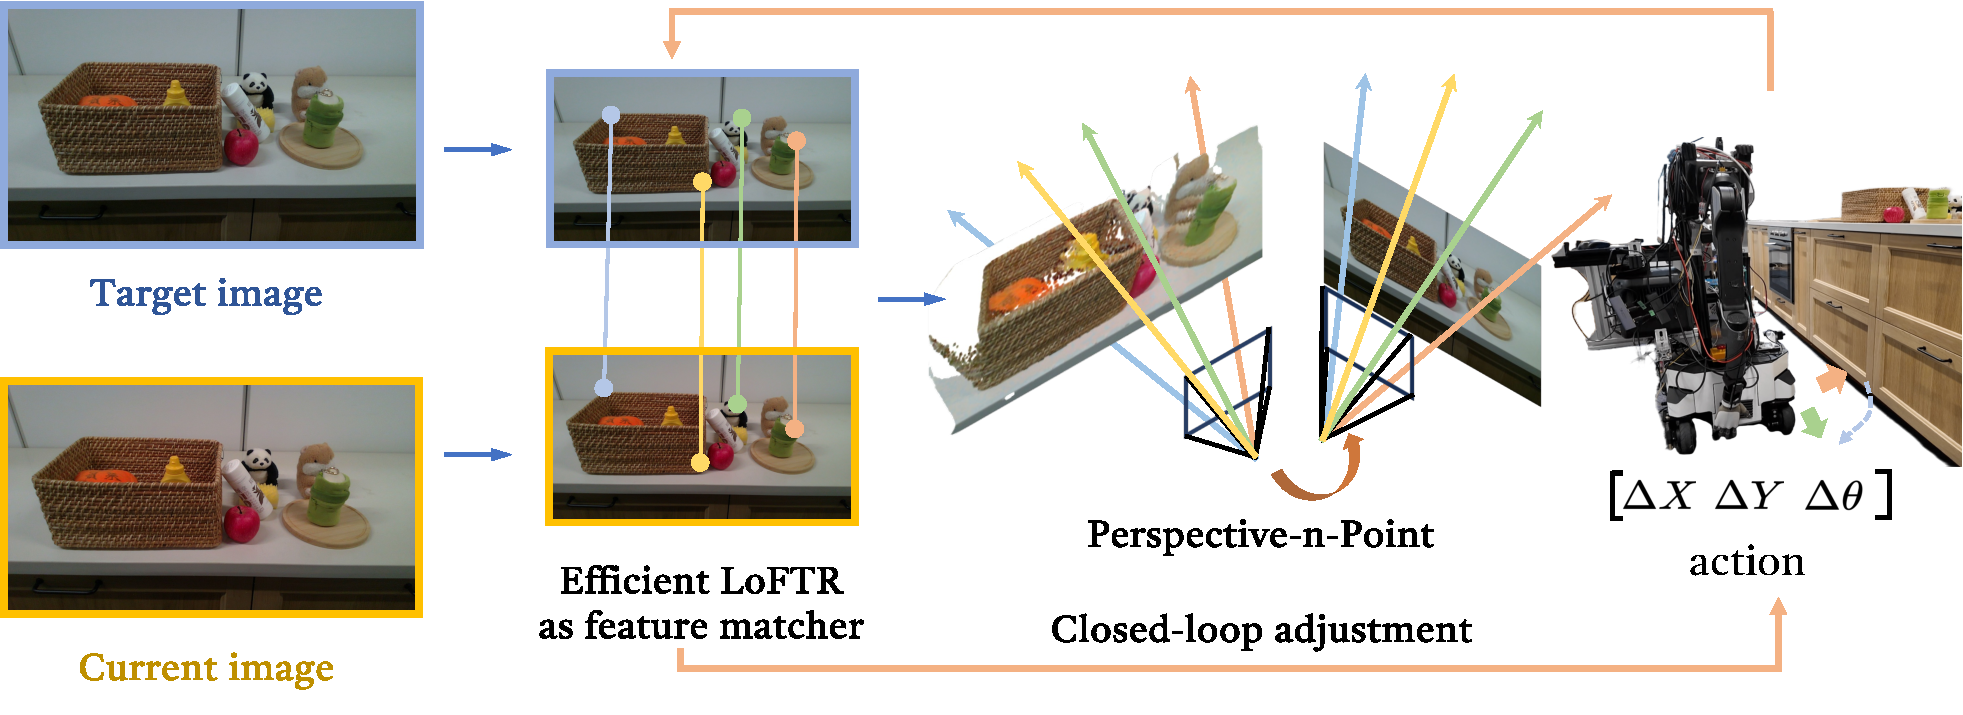
\includegraphics[width=1.0\linewidth]{figures/realtime-pnp_pic.pdf}
  \vspace{-15pt}
  \caption{ \textbf{The pipeline of closed-loop PnP localization.} We first employ the Efficient LoFTR  to extract dense visual correspondence, followed by estimating the transformation between the current frame and the goal location via solving the PnP problem. Subsequently, we use PID controller to execute the action. This entire process is executed in a closed-loop manner and continues iteratively until the spatial discrepancy between the robot's current pose and the goal falls below a predefined threshold.}
  \label{fig:realtime-pnp}
\end{figure*}

\subsection{Closed-loop PnP Localization}
For our mobile manipulation tasks, moderate discrepancies between the robot's final pose and the target pose can lead to the manipulation policy failing to finish the task. However, ViNT does not guarantee termination within a sufficiently tight error bound. To address this, we introduce a local refinement step after ViNT completes navigation: a closed-loop Perspective-n-Point~(PnP) localization algorithm is employed to adjust the robot pose, ensuring closer alignment with the target pose.

As shown in Figure~\ref{fig:realtime-pnp}, we first utilize the neural feature matching module Efficient LoFTR~\cite{wang2024efficient} to detect the correspondence between the current robot captured image $I_{c}$ and the goal image $I_{g}$. Next, the detected features are lifted to 3D space with respect to the robot's current coordinate frame by leveraging the camera intrinsic matrix $\mathbf{K}$ and the depth map $\mathbf{D_{c}}$. This yields $\mathbf{X_a}$, the 3D coordinates of the matched features in the current camera coordinate frame. According to Equation~\ref{eq: pnp}, we then leverage the RANSAC PnP~\cite{zuliani2009ransac} and refine PnP algorithm~\cite{madsen2004methods,eade2013gauss} to compute the relative rotation $\mathbf{R} \in \mathbb{R}^{3 \times 3}$ and translation $\mathbf{t} \in \mathbb{R}^{3}$ between the robot’s current viewpoint and the goal pose that can minimize the reprojection error $e=\left\|\tilde{\mathbf{P}}_{\mathbf{g}}-\mathbf{P}_{\mathbf{g}}\right\|_2^2 $: 

\begin{equation}
\label{eq: pnp}
\left[\begin{array}{c}
\tilde{\mathbf{P}}_{\mathbf{g}} \\
1
\end{array}\right]=\mathbf{K}[\mathbf{R} \mid \mathbf{t}]\left[\begin{array}{c}
\mathbf{X_a} \\
1
\end{array}\right] ,   
\end{equation}

where $\mathbf{P_{g}}$ denotes the pixel positions of the matched features at the goal image,  $\tilde{\mathbf{P}}_{\mathbf{g}}$ represents the reprojected positions. 
Adopting Efficient LoFTR can yield an inference rate of 16.7 Hz. By leveraging real-time feedback from PnP as the robot incrementally converges toward the target pose, we are able to iteratively refine the pose estimation, thus attaining more accurate visual correspondence. 

After getting the target pose calculated by our closed-loop PnP localization algorithm, we utilize a Proportional-Integral-Derivative~(PID) controller~\cite{willis1999proportional} to adjust the pose of our robot. The input of the controller is the instantaneous position and orientation error between the robot's desired state and its actual state. Since the mobile base exhibits limited control accuracy, we define separate PID controllers for reducing errors individually along the x and y directions, as well as for the yaw angle. Based on this multi-dimensional error input, the PID controller computes and outputs corresponding \textit{planar velocity commands} designed to minimize the error. These commands consist of velocities along the corresponding three directions. The velocity is computed as follows:

\begin{align}
v_j &= K_{p,j} e_j + K_{i,j} \int_{0}^{t} e_j(\tau)  d\tau + K_{d,j} \frac{de_j}{dt} 
\end{align}

where $j$ denotes a specific axis, $v_{j}$ is the velocity, $e_{j}$ represents the error term, and $K_{p,j}$, $K_{i,j}$, $K_{d,j}$ correspond to the proportional, integral, and derivative gain coefficients, respectively.

To address the characteristics of our omnidirectional chassis, which incurs additional displacement during wheel reorientation, we implement a sequential adjustment strategy, which prioritizes error correction in the order of x-direction, y-direction, yaw orientation. This staged compensation mitigates the coupling effects introduced by wheel realignment. 
